\section{Experimental Results}
\label{sec:results}

This section presents a rigorous empirical evaluation of the proposed Dueling Double Deep Q-Network (D3QN) sequential recommender system on the MovieLens 32M benchmark environment. Our experimental analysis is structured into three stages: (i) environment validation diagnostics under a uniform random policy to verify Markov Decision Process (MDP) well-posedness prior to reinforcement learning; (ii) an eight-configuration hyperparameter sensitivity study and training convergence analysis; and (iii) a comprehensive held-out test-set evaluation across $250$ unseen users comparing D3QN against heuristic, matrix factorization, and contextual bandit baselines at recommendation horizons $K=10$ and $K=20$.

\subsection{Random-Policy Environment Validation Diagnostics}
\label{subsec:random_diag}

Before initiating neural value-function approximation, we executed $N = 100$ diagnostic rollouts using a uniform random policy ($\pi_{\text{rand}}(a \mid s_t) = \mathcal{U}\{0, 1, \dots, 49\}$) over the $K_{\text{cand}} = 50$ candidate action slots at maximum horizon $H = 10$. In sequential reinforcement learning for recommendation, environment validation is critical to ensure that the reward shaping function does not suffer from trivial saturation or degenerate penalty collapse, that the termination condition creates a meaningful survival signal, and that all discrete candidate slots are reachable. Table~\ref{tab:random_diag} summarizes the resulting diagnostic statistics, and Fig.~\ref{fig:random_diag} illustrates the empirical distributions across all $875$ executed environment steps.

\begin{table}[t]
\centering
\caption{Random-Policy Environment Validation Diagnostic Metrics ($N = 100$ Episodes, Horizon $H = 10$)}
\label{tab:random_diag}
\footnotesize
\setlength{\tabcolsep}{5pt}
\begin{tabular}{@{}lc@{}}
\toprule
\textbf{Diagnostic Metric} & \textbf{Empirical Value} \\
\midrule
Diagnostic Episodes Executed ($N$) & $100$ \\
Total Environment Steps Executed & $875$ \\
Mean Episode Return ($\pm$ SD) & $1.1833 \pm 2.5468$ \\
Episode Return Range $[\min, \max]$ & $[-3.4769, \, 7.2058]$ \\
Mean Episode Length ($\pm$ SD) & $8.75 \pm 1.85\text{ steps}$ \\
Early Termination Rate ($5$ Consecutive Misses) & $37.0\%$ ($0.3700$) \\
Full $10$-Step Horizon Completion Rate & $63.0\%$ ($0.6300$) \\
Step-Level Hit Rate ($r_{u,i} \ge 3.5$) & $0.3053$ ($30.53\%$) \\
Mean Self-Information Novelty & $14.39\text{ bits}$ ($14.3890\text{ bits}$) \\
Repeat Action Selection Rate & $7.89\%$ ($0.0789$) \\
Unique Discrete Actions Sampled & $50 / 50$ ($100.0\%$) \\
\bottomrule
\end{tabular}
\end{table}

\begin{figure*}[t]
    \centering
    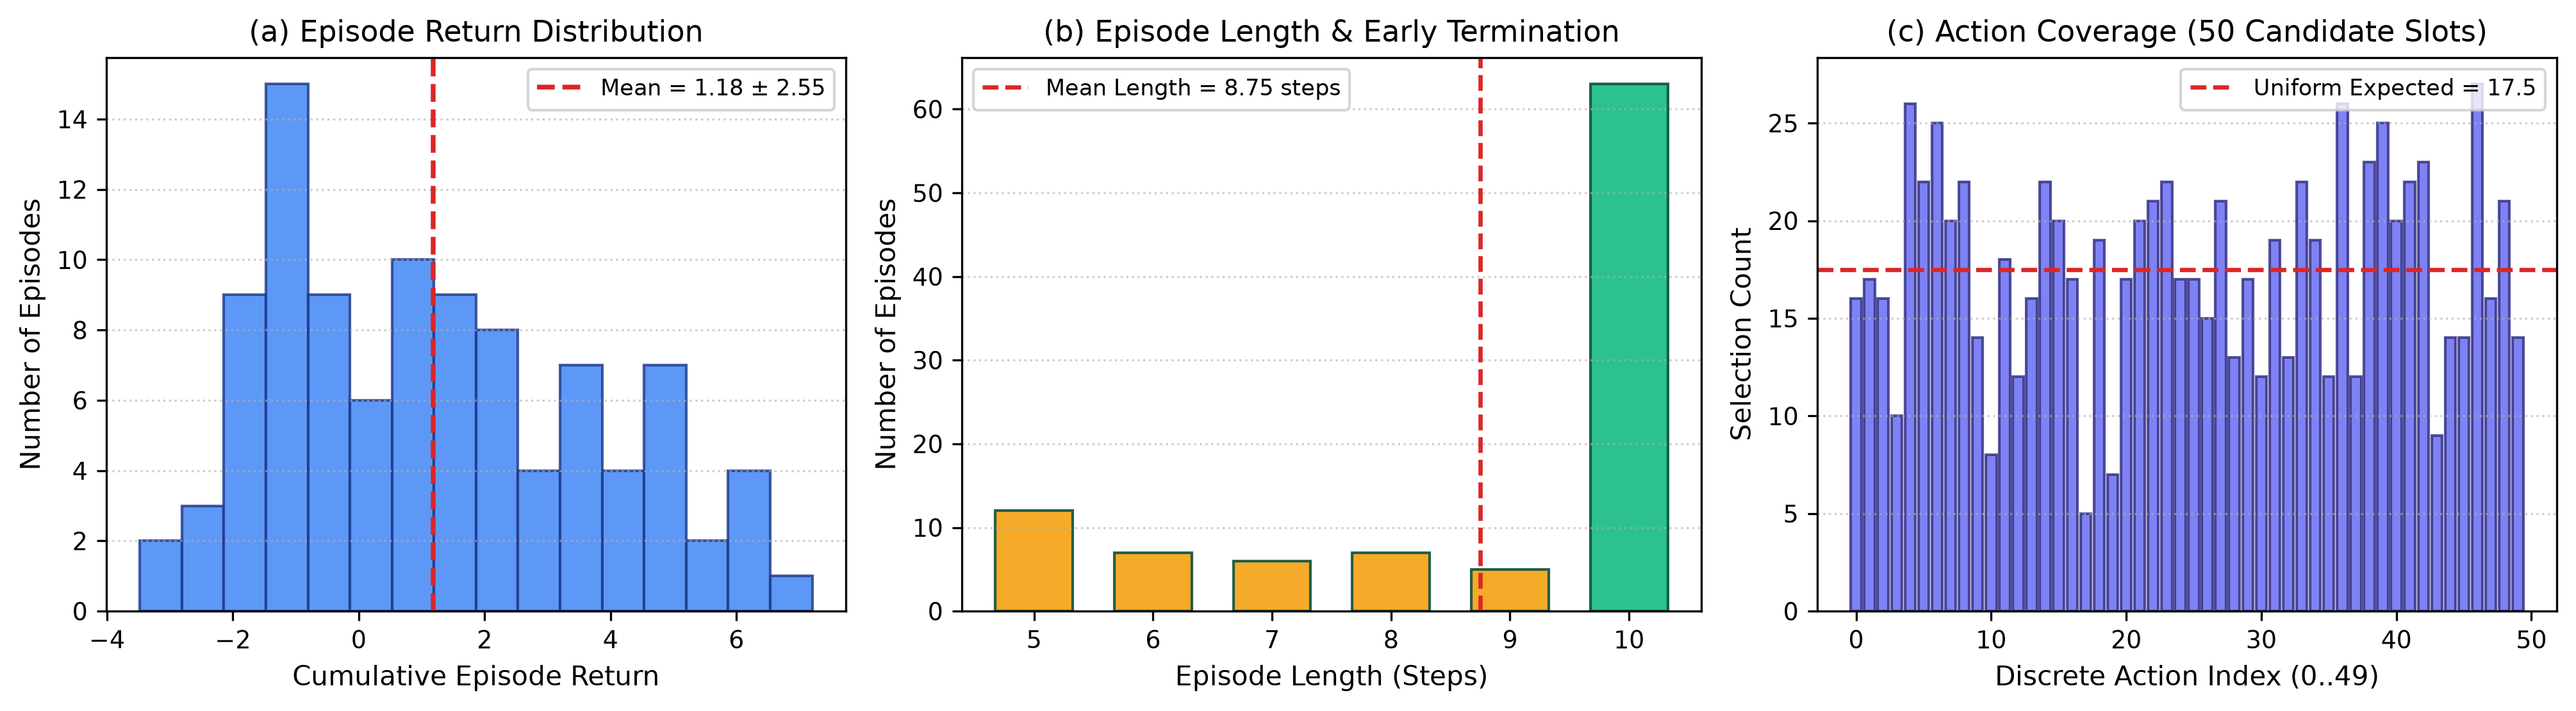
\includegraphics[width=0.96\textwidth]{figures/fig2_random_policy_diagnostics.png}
    \caption{Random-policy environment validation diagnostics across $N = 100$ episodes ($875$ total interaction steps): (a) Cumulative episode return distribution centered at $1.1833 \pm 2.5468$ over $[-3.4769, 7.2058]$, confirming a well-scaled reward landscape without trivial saturation; (b) Episode length histogram showing a $37.0\%$ early termination rate between steps $t=5$ and $t=9$ due to the $5$-consecutive-miss user abandonment rule versus $63.0\%$ full $10$-step horizon completion (mean length $8.75 \pm 1.85$ steps); and (c) Discrete action selection counts across all $50$ candidate slots relative to the theoretical uniform expectation ($17.5$ selections/slot), confirming $100\%$ action-space reachability ($50/50$ unique actions sampled).}
    \label{fig:random_diag}
\end{figure*}

Three structural properties emerge from Table~\ref{tab:random_diag} and Fig.~\ref{fig:random_diag}:
\begin{enumerate}
    \item \textbf{Well-Scaled Reward Landscape:} As shown in Fig.~\ref{fig:random_diag}(a), unguided uniform action selection yields a mean cumulative episode return of $1.1833 \pm 2.5468$, spanning a wide dynamic range from $-3.4769$ (sessions dominated by irrelevant recommendations, repetition penalties, and early abandonment) to $7.2058$ (fortuitous sequences of relevant and novel items). The step-level hit rate of $0.3053$ confirms that roughly $30.53\%$ of candidate pool slots correspond to positive user preferences, providing sufficient positive reinforcement signal for initial $\epsilon$-greedy exploration without making the task trivially solvable.
    \item \textbf{Active Session Abandonment Dynamics:} Fig.~\ref{fig:random_diag}(b) demonstrates that $37.0\%$ of random episodes terminate prematurely ($t \in \{5, 6, 7, 8, 9\}$) upon accumulating $5$ consecutive negative interactions, while $63.0\%$ survive to the full $H=10$ horizon, yielding a mean episode length of $8.75 \pm 1.85$ steps. This confirms that the user abandonment rule actively penalizes myopic or repetitive policies and incentivizes multi-step survival planning.
    \item \textbf{Complete Candidate Action Reachability:} Across the $875$ total steps, the random policy achieves a mean self-information novelty of $14.39$ bits ($14.3890$ bits), a repeat action rate of $7.89\%$ ($0.0789$), and samples all $50/50$ ($100\%$) discrete candidate slots around the theoretical uniform expectation of $875 / 50 = 17.5$ selections per slot (Fig.~\ref{fig:random_diag}(c)). This verifies that no candidate slots are structurally masked or unreachable prior to policy optimization.
\end{enumerate}

\subsection{Hyperparameter Sensitivity and Training Dynamics}
\label{subsec:hyperparam}

To systematically evaluate the stability and sample efficiency of our D3QN architecture, we conducted a controlled one-factor-at-a-time hyperparameter sensitivity study across eight configurations (\texttt{cfg1\_baseline} through \texttt{cfg8\_high\_l2}), each trained for $800$ episodes around the baseline setting ($\eta = 5 \times 10^{-4}$, $\gamma = 0.95$, $\delta_\epsilon = 0.995$, $\lambda_{L_2} = 10^{-5}$). Based on the sensitivity findings, we subsequently trained our Champion Tuned D3QN (\texttt{d3qn\_tuned}) for an extended schedule of $1{,}500$ episodes ($14{,}940$ total environment interaction steps). Table~\ref{tab:hyperparams} reports the complete validation metrics across all nine runs, while Fig.~\ref{fig:hyperparams} and Fig.~\ref{fig:exploration} illustrate the validation learning curves, hyperparameter sensitivity comparison, and internal value-function convergence dynamics.

\begin{table*}[t]
\centering
\caption{Hyperparameter Sensitivity Study ($800$ Episodes) and Champion Tuned D3QN ($1{,}500$ Episodes, $14{,}940$ Steps) on Validation Split ($H = 10$)}
\label{tab:hyperparams}
\resizebox{\textwidth}{!}{%
\begin{tabular}{@{}lccccccccccc@{}}
\toprule
\textbf{Configuration ID} & \textbf{LR $\eta$} & \textbf{Discount $\gamma$} & \textbf{Decay $\delta_\epsilon$} & \textbf{$L_2$ $\lambda_{L_2}$} & \textbf{Episodes} & \textbf{Final Val Return} & \textbf{Best Val Return} & \textbf{Val P@10} & \textbf{NDCG@10} & \textbf{MAP@10} & \textbf{Catalog Coverage} \\
\midrule
\texttt{cfg1\_baseline} & $5\times 10^{-4}$ & $0.95$ & $0.995$ & $10^{-5}$ & $800$ & $11.6598$ & $11.6598$ & $0.9490$ & $0.9610$ & $0.9348$ & $\mathbf{0.3586}$ ($\mathbf{35.86\%}$) \\
\texttt{cfg2\_high\_lr} & $1\times 10^{-3}$ & $0.95$ & $0.995$ & $10^{-5}$ & $800$ & $10.0227$ & $10.2034$ & $0.8410$ & $0.8609$ & $0.7799$ & $0.3433$ ($34.33\%$) \\
\texttt{cfg3\_low\_lr} & $1\times 10^{-4}$ & $0.95$ & $0.995$ & $10^{-5}$ & $800$ & $9.7503$ & $9.7503$ & $0.8220$ & $0.8630$ & $0.7758$ & $0.3533$ ($35.33\%$) \\
\texttt{cfg4\_gamma\_090} & $5\times 10^{-4}$ & $0.90$ & $0.995$ & $10^{-5}$ & $800$ & $11.3549$ & $11.4411$ & $0.9280$ & $0.9470$ & $0.9093$ & $0.3528$ ($35.28\%$) \\
\texttt{cfg5\_gamma\_099} & $5\times 10^{-4}$ & $0.99$ & $0.995$ & $10^{-5}$ & $800$ & $11.0368$ & $11.0368$ & $0.9030$ & $0.9196$ & $0.8655$ & $0.3454$ ($34.54\%$) \\
\texttt{cfg6\_fast\_eps} & $5\times 10^{-4}$ & $0.95$ & $0.990$ & $10^{-5}$ & $800$ & $11.5811$ & $11.5811$ & $0.9420$ & $0.9515$ & $0.9179$ & $0.3444$ ($34.44\%$) \\
\texttt{cfg7\_slow\_eps} & $5\times 10^{-4}$ & $0.95$ & $0.998$ & $10^{-5}$ & $800$ & $11.5718$ & $11.6073$ & $0.9360$ & $0.9438$ & $0.9085$ & $0.3470$ ($34.70\%$) \\
\texttt{cfg8\_high\_l2} & $5\times 10^{-4}$ & $0.95$ & $0.995$ & $10^{-4}$ & $800$ & $11.4517$ & $11.4517$ & $0.9350$ & $0.9514$ & $0.9153$ & $0.3486$ ($34.86\%$) \\
\midrule
\texttt{d3qn\_tuned} (Champion) & $5\times 10^{-4}$ & $0.95$ & $0.995$ & $10^{-5}$ & $1{,}500$ & $\mathbf{12.1668}$ & $\mathbf{12.2125}$ & $\mathbf{0.9770}$ & $\mathbf{0.9807}$ & $\mathbf{0.9684}$ & $0.3465$ ($34.65\%$) \\
\bottomrule
\end{tabular}%
}
\end{table*}

\begin{figure*}[t]
    \centering
    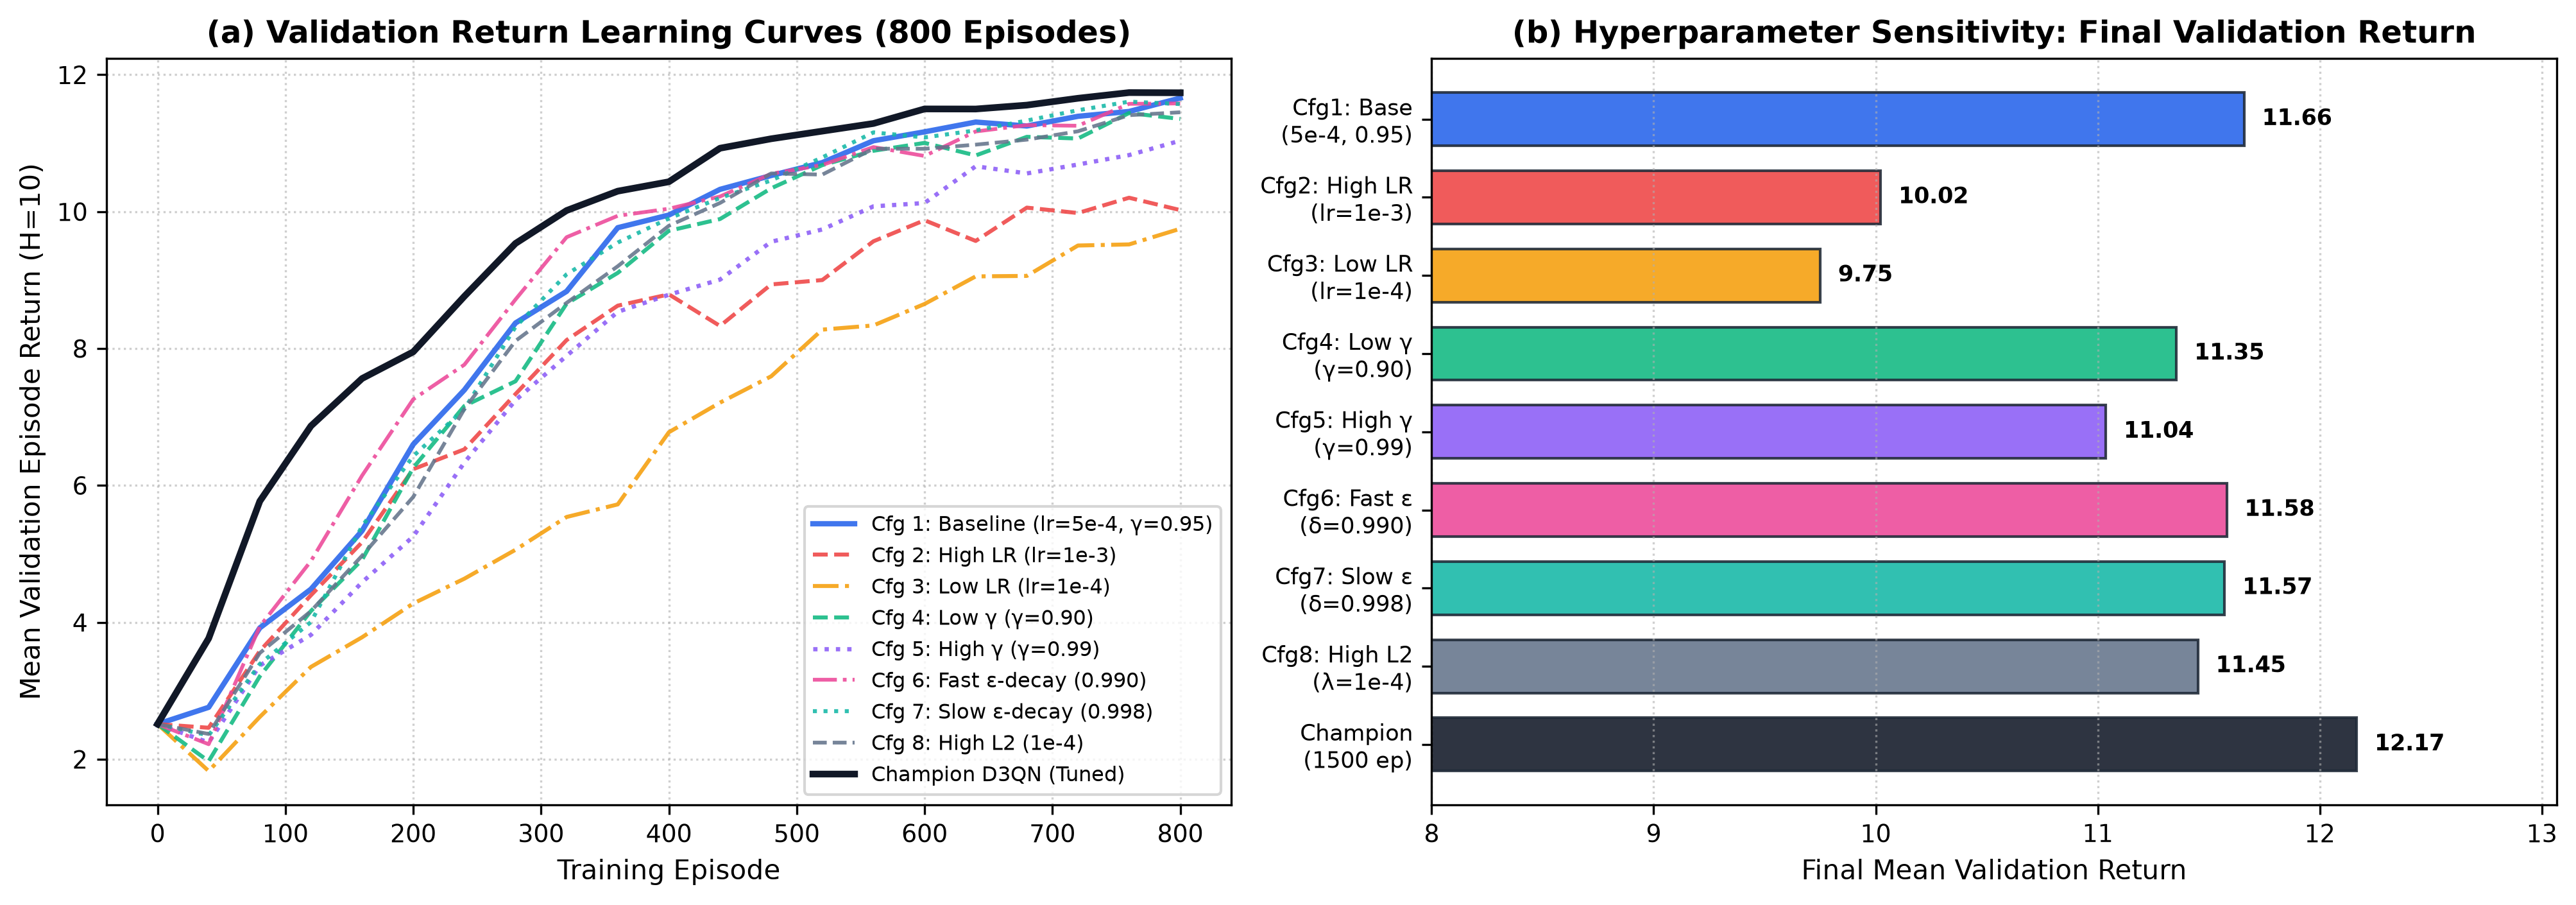
\includegraphics[width=0.96\textwidth]{figures/fig3_hyperparameter_learning_curves.png}
    \caption{Hyperparameter sensitivity analysis across $800$ training episodes and extended Champion D3QN training ($1{,}500$ episodes): (a) Mean validation episode return learning curves ($H=10$, evaluated every $40$ episodes at $\epsilon=0$), showing rapid convergence for $\eta = 5 \times 10^{-4}$ and $\gamma = 0.95$ compared to high-LR oscillation ($\eta = 10^{-3}$) and low-LR under-fitting ($\eta = 10^{-4}$); and (b) Final validation return comparison across all eight $800$-episode configurations and the Champion Tuned D3QN ($12.1668$).}
    \label{fig:hyperparams}
\end{figure*}

\begin{figure*}[t]
    \centering
    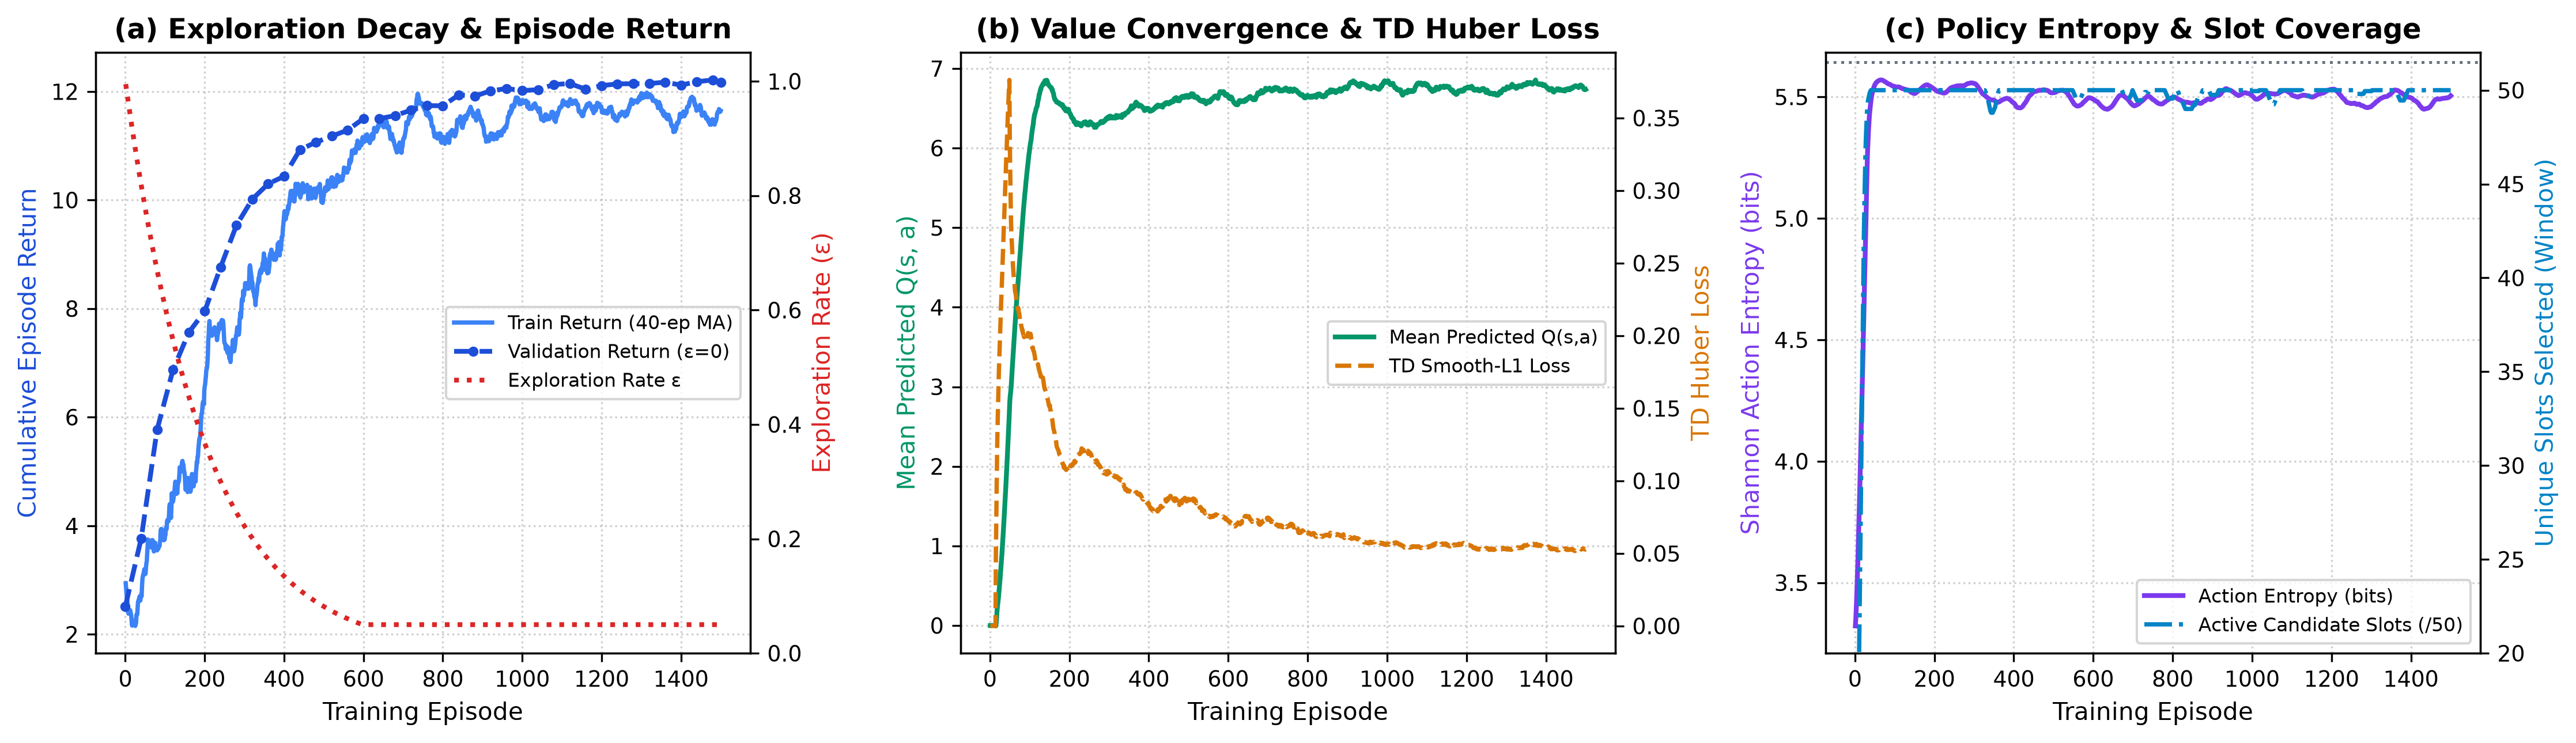
\includegraphics[width=0.96\textwidth]{figures/fig4_exploration_dynamics.png}
    \caption{Internal training and exploration dynamics of the Champion Tuned D3QN across $1{,}500$ episodes ($14{,}940$ steps): (a) Co-evolution of the $40$-episode moving-average training return, greedy validation return ($\epsilon=0$), and exponential exploration rate $\epsilon_t$; (b) Stabilization of mean predicted action-values $Q(s,a)$ alongside the monotonic decay of temporal-difference (TD) Smooth-$L_1$ (Huber) loss; and (c) Policy Shannon action entropy (bits) and sliding-window active candidate slot coverage ($50/50$ slots).}
    \label{fig:exploration}
\end{figure*}

\paragraph{Learning Rate Sensitivity ($\eta$)}
As evidenced in Table~\ref{tab:hyperparams} and Fig.~\ref{fig:hyperparams}(a), the AdamW step size $\eta$ exerts the strongest influence on policy convergence. The moderate learning rate $\eta = 5 \times 10^{-4}$ (\texttt{cfg1\_baseline}) achieves the highest $800$-episode performance across all ranking and return criteria, reaching a final validation return of $11.6598$, P@10 of $0.9490$, NDCG@10 of $0.9610$, MAP@10 of $0.9348$, and the highest validation catalog coverage of $0.3586$ ($35.86\%$). Increasing the step size to $\eta = 10^{-3}$ (\texttt{cfg2\_high\_lr}) degrades final validation return to $10.0227$ (best $10.2034$, NDCG@10 of $0.8609$, MAP@10 of $0.7799$) because aggressive gradient updates amplify moving-target non-stationarity in the Polyak-averaged target network, inducing target $Q$-value overshoot and mid-training return oscillations after episode $350$. Conversely, reducing the learning rate to $\eta = 10^{-4}$ (\texttt{cfg3\_low\_lr}) yields the lowest validation return of $9.7503$ (P@10 of $0.8220$, NDCG@10 of $0.8630$, MAP@10 of $0.7758$), as parameter updates proceed too slowly to separate the advantage stream $A_\theta(s,a)$ across the $50$ candidate slots within an $800$-episode budget.

\paragraph{Discount Factor Sensitivity ($\gamma$)}
Varying the Bellman discount factor confirms the necessity of multi-step trajectory planning over myopic or over-extended horizons. Setting $\gamma = 0.95$ (\texttt{cfg1\_baseline}, validation return $11.6598$) outperforms both a more myopic discount of $\gamma = 0.90$ (\texttt{cfg4\_gamma\_090}, final validation return $11.3549$, best $11.4411$, P@10 of $0.9280$, NDCG@10 of $0.9470$) and a near-undiscounted $\gamma = 0.99$ (\texttt{cfg5\_gamma\_099}, final validation return $11.0368$, P@10 of $0.9030$, NDCG@10 of $0.9196$). Under $\gamma = 0.90$, the effective planning horizon $(1-\gamma)^{-1} = 10$ steps heavily discounts late-session diversity and novelty rewards, leading to premature genre saturation. Conversely, $\gamma = 0.99$ propagates long-horizon bootstrap variance across episodes of length $H=10$, destabilizing Bellman target estimation and depressing MAP@10 to $0.8655$.

\paragraph{Exploration Schedule ($\delta_\epsilon$) and $L_2$ Regularization ($\lambda_{L_2}$)}
Faster exploration decay $\delta_\epsilon = 0.990$ (\texttt{cfg6\_fast\_eps}) accelerates early validation gains between episodes $100$ and $350$ (Fig.~\ref{fig:hyperparams}(a)) and finishes at $11.5811$ (NDCG@10 of $0.9515$), but its premature transition to greedy exploitation slightly narrows catalog coverage to $0.3444$ ($34.44\%$). Slower decay $\delta_\epsilon = 0.998$ (\texttt{cfg7\_slow\_eps}) maintains prolonged stochasticity, achieving a best validation return of $11.6073$ (final $11.5718$, NDCG@10 of $0.9438$) and higher validation novelty ($15.4025$ bits), at the cost of slower initial convergence. Stronger weight decay $\lambda_{L_2} = 10^{-4}$ (\texttt{cfg8\_high\_l2}) regularizes network weights slightly too aggressively, yielding a final validation return of $11.4517$ (P@10 of $0.9350$, NDCG@10 of $0.9514$) compared to $\lambda_{L_2} = 10^{-5}$ ($11.6598$).

\paragraph{Champion Tuned D3QN Convergence and Sample Efficiency}
Retaining the optimal hyperparameters ($\eta = 5 \times 10^{-4}$, $\gamma = 0.95$, $\delta_\epsilon = 0.995$, $\lambda_{L_2} = 10^{-5}$) over $1{,}500$ episodes ($14{,}940$ steps) allows the Champion Tuned D3QN (\texttt{d3qn\_tuned}) to reach a final validation return of $12.1668$ (peaking at a best validation return of $12.2125$ at episode $1{,}480$ / step $14{,}740$), alongside a validation P@10 of $0.9770$, R@10 of $0.5147$, NDCG@10 of $0.9807$, MAP@10 of $0.9684$, HR@10 of $1.0000$, catalog coverage of $0.3465$ ($34.65\%$), and mean novelty of $15.5923$ bits. As shown in Fig.~\ref{fig:exploration}(a), the agent exhibits exceptional sample efficiency: starting from an untrained return of $2.5138$ at step $0$ (which already exceeds the static Greedy FunkSVD baseline of $1.3609$ due to hybrid candidate generation), the D3QN policy surpasses the Myopic Contextual Bandit return threshold ($10.4924$) after just $3{,}940$ interaction steps ($400$ episodes, validation return $10.4368 \to 10.9268$ at episode $440$). Fig.~\ref{fig:exploration}(b) confirms that Double DQN decoupling and dueling value-advantage decomposition prevent maximization bias: the mean predicted $Q(s,a)$ converges smoothly to an asymptotic plateau near $6.75$ while the TD Smooth-$L_1$ (Huber) loss decays monotonically from an initial peak of $0.38$ to a stable floor of $0.05$. Simultaneously, Fig.~\ref{fig:exploration}(c) shows that policy Shannon entropy stabilizes near $5.50$ bits (close to the $\log_2 50 \approx 5.6439$-bit uniform ceiling across users) while utilizing all $50/50$ candidate slots.

\subsection{Test-Set Evaluation and Baseline Comparison}
\label{subsec:test_eval}

We evaluated the locked Champion D3QN policy ($\epsilon = 0$) against five baselines across all $250$ held-out test users under two recommendation horizons: $K = 10$ ($H = 10$ steps) and $K = 20$ ($H = 20$ steps). The evaluated baselines span unguided selection (\texttt{Random}), non-personalized and additive-bias heuristics (\texttt{Popularity} and \texttt{Bias} $\mu + b_u + b_i$), our Workshop~1 matrix factorization model deployed sequentially (\texttt{Greedy FunkSVD}), and a neural contextual bandit trained with identical state-action representations but zero lookahead (\texttt{Myopic Contextual Bandit}, $\gamma = 0$). Table~\ref{tab:test_comparison} details the complete test-set performance across nine evaluation metrics, and Fig.~\ref{fig:test_comparison} visualizes the top-$10$ ranking accuracy and the multi-objective accuracy--coverage--novelty trade-off.

\begin{table*}[t]
\centering
\caption{Comprehensive Test-Set Evaluation Across $250$ Held-Out Users at Horizons $K = 10$ and $K = 20$}
\label{tab:test_comparison}
\resizebox{\textwidth}{!}{%
\begin{tabular}{@{}clccccccccc@{}}
\toprule
\textbf{Horizon} & \textbf{Policy / Model} & \textbf{Mean Return ($\pm$ SD)} & \textbf{P@$K$} & \textbf{R@$K$} & \textbf{NDCG@$K$} & \textbf{MAP@$K$} & \textbf{HR@$K$} & \textbf{Catalog Cov. (\%)} & \textbf{Novelty (bits)} & \textbf{ILD} \\
\midrule
$K = 10$ & Random & $2.6805 \pm 2.4628$ & $0.3412$ & $0.1798$ & $0.3480$ & $0.1949$ & $0.9080$ & $\mathbf{43.48\%}$ & $14.7450$ & $\mathbf{0.9664}$ \\
$K = 10$ & Bias ($\mu + b_u + b_i$) & $-0.0451 \pm 1.7509$ & $0.1188$ & $0.0626$ & $0.1345$ & $0.0658$ & $0.5000$ & $7.93\%$ & $14.5493$ & $0.8030$ \\
$K = 10$ & Popularity & $-1.4121 \pm 0.6586$ & $0.0392$ & $0.0207$ & $0.0551$ & $0.0240$ & $0.2800$ & $4.02\%$ & $8.8545$ & $0.6864$ \\
$K = 10$ & Greedy FunkSVD (Workshop 1) & $1.3609 \pm 2.1743$ & $0.2524$ & $0.1330$ & $0.2785$ & $0.1519$ & $0.7920$ & $17.25\%$ & $13.0788$ & $0.8653$ \\
$K = 10$ & Myopic Contextual Bandit ($\gamma=0$) & $10.4924 \pm 1.8230$ & $0.8708$ & $0.4589$ & $0.8924$ & $0.8253$ & $\mathbf{1.0000}$ & $34.35\%$ & $14.9406$ & $0.4215$ \\
$K = 10$ & \textbf{D3QN (Ours, $\gamma=0.95$)} & $\mathbf{12.3674 \pm 0.8253}$ & $\mathbf{0.9792}$ & $\mathbf{0.5160}$ & $\mathbf{0.9818}$ & $\mathbf{0.9692}$ & $\mathbf{1.0000}$ & $36.64\%$ & $\mathbf{17.9613}$ & $0.2731$ \\
\midrule
$K = 20$ & Random & $4.3195 \pm 3.2988$ & $0.2954$ & $0.3113$ & $0.3274$ & $0.1610$ & $0.9280$ & $59.19\%$ & $14.5759$ & $\mathbf{0.9734}$ \\
$K = 20$ & Bias ($\mu + b_u + b_i$) & $-0.0470 \pm 1.9373$ & $0.0766$ & $0.0807$ & $0.1028$ & $0.0415$ & $0.5000$ & $12.36\%$ & $14.3013$ & $0.8009$ \\
$K = 20$ & Popularity & $-1.4224 \pm 0.7428$ & $0.0210$ & $0.0222$ & $0.0379$ & $0.0132$ & $0.2800$ & $4.51\%$ & $8.8756$ & $0.6862$ \\
$K = 20$ & Greedy FunkSVD (Workshop 1) & $1.4372 \pm 2.6229$ & $0.1616$ & $0.1704$ & $0.2127$ & $0.0959$ & $0.7920$ & $25.10\%$ & $13.2404$ & $0.8742$ \\
$K = 20$ & Myopic Contextual Bandit ($\gamma=0$) & $16.5601 \pm 4.1903$ & $0.7262$ & $0.7654$ & $0.8068$ & $0.6852$ & $\mathbf{1.0000}$ & $57.42\%$ & $15.9685$ & $0.6061$ \\
$K = 20$ & \textbf{D3QN (Ours, $\gamma=0.95$)} & $\mathbf{20.1006 \pm 1.8207}$ & $\mathbf{0.8398}$ & $\mathbf{0.8849}$ & $\mathbf{0.9167}$ & $\mathbf{0.8605}$ & $\mathbf{1.0000}$ & $\mathbf{60.35\%}$ & $\mathbf{17.2745}$ & $0.4698$ \\
\bottomrule
\end{tabular}%
}
\end{table*}

\begin{figure*}[t]
    \centering
    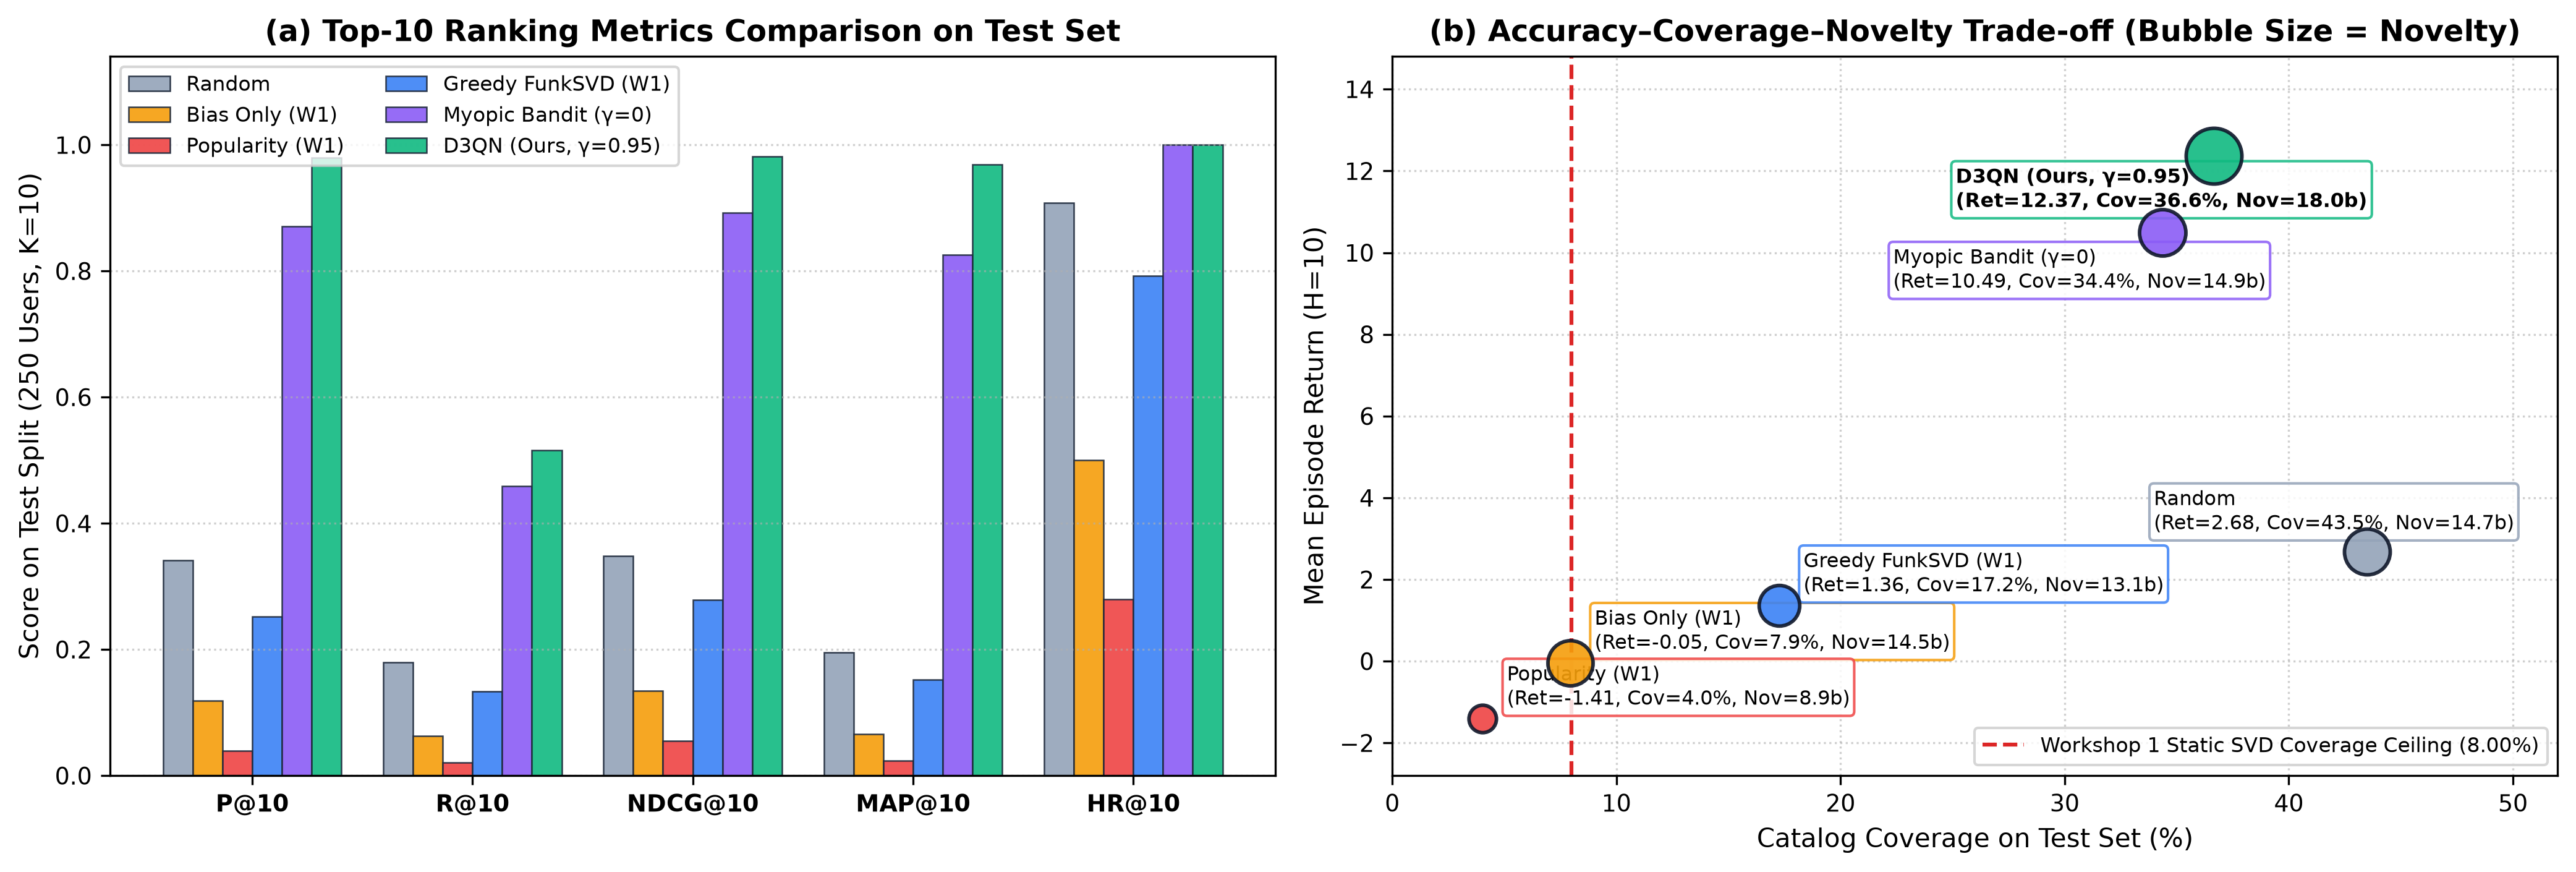
\includegraphics[width=0.96\textwidth]{figures/fig5_test_metrics_comparison.png}
    \caption{Test-set evaluation across $250$ held-out users: (a) Top-$10$ ranking metrics comparison (P@10, R@10, NDCG@10, MAP@10, and HR@10), illustrating the progression from static Workshop~1 baselines (\texttt{Popularity}, \texttt{Bias Only}, \texttt{Greedy FunkSVD}) to the \texttt{Myopic Bandit} ($\gamma=0$) and our proposed \texttt{D3QN} ($\gamma=0.95$); and (b) Multi-objective accuracy--coverage--novelty trade-off at $K=10$ (bubble area proportional to self-information novelty in bits), showing how D3QN simultaneously maximizes mean return ($12.3674$) and novelty ($17.96$ bits) while expanding catalog coverage to $36.64\%$ ($4.58\times$ the $8.00\%$ Workshop~1 static SVD ceiling).}
    \label{fig:test_comparison}
\end{figure*}

\paragraph{Superior Sequential Ranking and Trajectory Return}
Across both evaluation horizons in Table~\ref{tab:test_comparison}, \texttt{D3QN (Ours)} substantially outperforms every baseline on cumulative return, ranking precision, discounted ranking quality, and item novelty. At $K = 10$, D3QN achieves a mean episode return of $12.3674 \pm 0.8253$ (with $100\%$ of sessions completing the full $10.0$-step horizon), P@10 of $0.9792$, R@10 of $0.5160$, NDCG@10 of $0.9818$, MAP@10 of $0.9692$, and HR@10 of $1.0000$. When the evaluation horizon doubles to $K = 20$ without retraining, D3QN maintains full $20.0$-step session survival across all $250$ users, reaching a mean return of $20.1006 \pm 1.8207$, P@20 of $0.8398$, R@20 of $0.8849$, NDCG@20 of $0.9167$, MAP@20 of $0.8605$, and HR@20 of $1.0000$ (while its top-$10$ prefix metrics inside the $H=20$ rollout reach P@10 $= 0.9796$, R@10 $= 0.5162$, NDCG@10 $= 0.9825$, and MAP@10 $= 0.9707$).

\paragraph{Failure of Static Heuristics and Greedy Matrix Factorization in Sequential Interaction}
A striking empirical finding in Table~\ref{tab:test_comparison} and Fig.~\ref{fig:test_comparison}(a) is the severe degradation of static recommenders when deployed in an interactive sequential environment. In our Workshop~1 static offline evaluation, matrix factorization (\texttt{FunkSVD}) achieved a competitive rating prediction accuracy of $\text{RMSE} = 0.8041$ ($0.8128$ on the global unpooled split), yet suffered from the classic accuracy--ranking mismatch: on global all-item ranking, \texttt{Popularity} achieved NDCG@10 of $0.6726$ versus \texttt{FunkSVD}'s $0.5881$ ($0.2460$ on the Workshop~1 static test split with P@10 $= 0.2190$, R@10 $= 0.1450$, MAP@10 $= 0.1440$, HR@10 $= 0.5620$, novelty $= 9.83$ bits, and catalog coverage capped at only $8.00\%$). In the sequential MDP environment of Workshop~3, repeatedly selecting head items (\texttt{Popularity}) or static baseline scores (\texttt{Bias} $\mu + b_u + b_i$) fails to adapt to user feedback and rapidly triggers the $5$-consecutive-miss abandonment rule: at $K=10$, \texttt{Popularity} averages only $5.8720$ steps per episode with a negative mean return of $-1.4121 \pm 0.6586$ (P@10 $= 0.0392$, NDCG@10 $= 0.0551$, coverage $= 4.02\%$, novelty $= 8.8545$ bits), while \texttt{Bias} terminates at $6.9360$ steps with a mean return of $-0.0451 \pm 1.7509$ (P@10 $= 0.1188$, NDCG@10 $= 0.1345$, coverage $= 7.93\%$). Even \texttt{Greedy FunkSVD}, which ranks candidates strictly by static dot-product predictions $\hat{r}_{u,i}$ without state evolution, achieves a mean return of only $1.3609 \pm 2.1743$ at $K=10$ (mean length $8.5000$ steps, P@10 $= 0.2524$, R@10 $= 0.1330$, NDCG@10 $= 0.2785$, MAP@10 $= 0.1519$, coverage $= 17.25\%$) and $1.4372 \pm 2.6229$ at $K=20$ (mean length $11.7200$ steps, P@20 $= 0.1616$, NDCG@20 $= 0.2127$). Because \texttt{Greedy FunkSVD} lacks negative preference suppression and novelty planning, it underperforms even the memoryless \texttt{Random} policy ($2.6805$ at $K=10$ and $4.3195$ at $K=20$), which naturally avoids deterministic failure loops through uniform slot sampling.

\paragraph{Value of Multi-Step Bellman Planning ($\gamma = 0.95$ vs.\ Myopic Bandit $\gamma = 0$)}
Comparing \texttt{D3QN} ($\gamma = 0.95$) against the \texttt{Myopic Contextual Bandit} ($\gamma = 0$) isolates the exact contribution of multi-step Bellman lookahead, since both models observe the identical $250$-dimensional state representation across the $50$ candidate slots. At $K=10$, multi-step planning increases mean episode return by $+17.87\%$ ($12.3674$ vs.\ $10.4924$) while cutting return standard deviation more than in half ($0.8253$ vs.\ $1.8230$), boosting P@10 from $0.8708$ to $0.9792$ ($+10.84$ percentage points), NDCG@10 from $0.8924$ to $0.9818$ ($+8.94$ points), and MAP@10 from $0.8253$ to $0.9692$ ($+14.39$ points). The advantage of long-horizon planning becomes even more pronounced at $K = 20$: while the myopic bandit begins to exhaust obvious high-scoring candidates and suffers early terminations (mean length dropping to $19.5200$ steps, return $16.5601 \pm 4.1903$, P@20 $= 0.7262$, NDCG@20 $= 0.8068$, MAP@20 $= 0.6852$), D3QN sustains $20.0$-step completion across every user and achieves a $+21.38\%$ higher return ($20.1006 \pm 1.8207$), $+11.36$ points higher P@20 ($0.8398$), $+10.99$ points higher NDCG@20 ($0.9167$), and $+17.53$ points higher MAP@20 ($0.8605$).

\paragraph{Breaking the Workshop 1 Catalog Coverage and Novelty Ceiling}
Finally, Fig.~\ref{fig:test_comparison}(b) highlights how sequential reinforcement learning resolves the catalog concentration bottleneck identified in Workshop~1. Whereas static FunkSVD recommendations were confined to just $8.00\%$ of the catalog with a mean novelty of $9.83$ bits, D3QN expands test-set catalog coverage to $36.64\%$ at $K=10$---a $4.58\times$ expansion over Workshop~1's $8.00\%$ ceiling---while elevating mean self-information novelty to $17.96$ bits ($17.9613$ bits vs.\ $14.9406$ bits for the Myopic Bandit and $13.0788$ bits for Greedy FunkSVD). At $K=20$, D3QN expands catalog coverage further to $60.35\%$ ($0.6035$) with $17.2745$ bits of novelty, surpassing even the uniform \texttt{Random} policy ($59.19\%$) because \texttt{Random} loses $4.0$ steps per episode on average to early abandonment ($16.0$ vs.\ $20.0$ steps). Although D3QN exhibits a lower intra-list diversity ($\text{ILD} = 0.2731$ at $K=10$ and $0.4698$ at $K=20$) than unguided \texttt{Random} ($\text{ILD} = 0.9664$ and $0.9734$), this reflects purposeful preference alignment: rather than scattering recommendations across disliked genres, D3QN concentrates within each user's positively reinforced latent taste cluster while leveraging the novelty bonus to surface high-information long-tail films across the broader catalog.
